\section{Description of the Experiment}

\begin{figure}[H]
\centering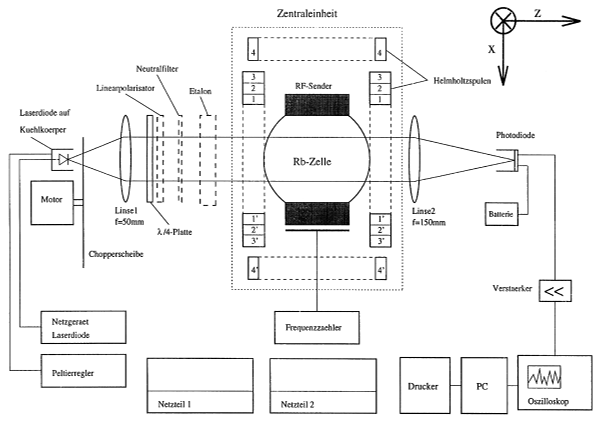
\includegraphics[width=\textwidth]{BilderTheo/Aufbau.png}
\caption{The experimental setup}
\end{figure}

The experimental setup mainly consists of an optical bench with a spherical \textbf{glass cell} at the center containing Rubidium and Krypton as a buffer gas. At the one end of the optical bench is a \textbf{laser diode} and a \textbf{collimator lens} in order to have a parallel beam, at the other end is a \textbf{photo diode} with a \textbf{collecting lens} in front of it. The laser diode's light's frequency can be changed by increasing or decreasing the current or the temperature of it, which is why there are a \textbf{Peltier element} and a \textbf{current regulator} connected to the laser. The photo diode is connected to a \textbf{preamplifier}, which leads to an \textbf{oscilloscope} and a \textbf{computer} in order to be able to register the signals. Into the optical path one can insert an \textbf{etalon}, \textbf{neutral filters} and a \textbf{quarter-wave plate}. The latter polarizes the light circularly and is needed for the optical pumping process, since the Rubidium atoms need to be stimulated by circular-polarized light in this case. The neutral filters can weaken the laser beam's intensity and can be used if for example the photo diode is overloaded and are also used in Dehmelt's method for the determination of the relaxation time, as will be explained later in chapter 4. The etalon is used to determine the time-frequency relationship on the oscilloscope. It is a Fabry-Pérot interferometer with a fixed width, which means that the distance between two peaks (constructive interference) in its spectrum is fixed.\footnote{It has a free spectral range of $(9924 \pm 30)\ MHz$}. Finally, we have 4 different \textbf{Helmholtz coils} and a \textbf{radio frequency emitter (RF)}. The Helmholtz coils are needed to generate magnetic fields for the different measuring methods. We will explain which coil we need and why we need it in each of the corresponding measurements in chapter 4. The radio frequency emitter will be needed for the double resonance method and its use will also be explained there. For Franzen's method for the determination of the relaxation time, we also need a \textbf{chopper disc}, which is a spinning disc with holes in it, in order to periodically cut off the laser beam and then letting it through again, which makes it a stroboscope.

\clearpage